% ============================================================================
%  SUPPLEMENTARY MATERIAL — 3DV 2027 submission (due 2026-09-02)
%  Build:  cd paper2 && tectonic supplementary.tex
%
%  Contents: the two former in-paper appendices, moved here for the 3DV page
%  limit (author decision anticipated in appendix_companion.tex since
%  2026-07-09). Section files are shared with the old single-document build;
%  their % src: grounding comments are unchanged. Counters are S-prefixed so
%  the main paper can cite "suppl. Table S1 / Fig. S1" unambiguously.
%  No \cite here, so no bibliography is emitted.
% ============================================================================
\documentclass[10pt,twocolumn,letterpaper]{article}

\usepackage[review]{cvpr}      % same anonymous review mode as the paper
% \usepackage{cvpr}              % camera-ready

\usepackage[dvipsnames]{xcolor}
\definecolor{cvprblue}{rgb}{0.21,0.49,0.74}
\usepackage[pagebackref,breaklinks,colorlinks,citecolor=cvprblue]{hyperref}

%%%%%%%%% PAPER ID — keep in sync with main.tex
\def\paperID{*****}
\def\confName{3DV\xspace}
\def\confYear{2027\xspace}

\graphicspath{{figures/}}
\newcommand{\TODO}[1]{\textcolor{red}{\textbf{[\,TODO: #1\,]}}}

\title{Supplementary Material for\\
       Topology-Correcting Differentiable Triangle-Soup Reconstruction\\
       via Persistent Homology}

% DOUBLE-BLIND: anonymous in review mode, same as main.tex.
\author{}

\begin{document}
\maketitle

% S-prefixed counters: the main paper refers to these as Table S1-S3, Fig. S1.
\appendix
\renewcommand{\thetable}{S\arabic{table}}
\renewcommand{\thefigure}{S\arabic{figure}}

\appendix
\section{The allocation-channel study, in brief}
\label{app:companion}

% Added 2026-07-09 for submit-first self-containment: the three facts this
% paper uses from the companion manuscript are restated here WITH their
% numbers, so reviewers can audit the argument from this document alone.
% src: figures/summary.md a.k.a. blindness_results.json (Phase 1);
%      h2_unified/report/results.json (voids, 5 paired seeds);
%      crossover/report/results.json (torus incl. B5).
% NOTE(author): at venues with strict page limits this appendix moves to the
% supplementary material unchanged, alongside the companion PDF itself.

This appendix restates, with their numbers, the three facts of the companion
study~\citep{chongpermwattanapol2026spread} that this paper builds on.

\paragraph{(1) Geometric metrics are topology-blind.} Three constructed
cases each pit a topologically correct candidate A against a wrong one B
whose geometry is bisection-matched, making Chamfer \emph{equal by
construction} (40k samples, metrics normalized by the ground-truth bounding
diagonal). A thin handle (genus $0{\to}1$): Chamfer $0.916\%$ for both,
discriminating bottleneck $0.030$ vs ${\approx}0$. A thin bridge merging two
components: Chamfer $0.628\%$ both, bottleneck $40\times$ apart ($.0574$ vs
$.0014$). A punctured void: Chamfer $0.977\%$ both, bottleneck $35\times$
apart ($.1385$ vs $.0040$). In the first two cases Hausdorff$_{95}$ actually
\emph{prefers} the wrong candidate. Chamfer cannot tell a benign bump from a
destroyed void; the persistence metric separates them by more than an order
of magnitude.
% src: figures/summary.md (Phase-1 result table, 3/3 gate)

\paragraph{(2) The prior arms, and why voids are ``width-primary''.} The
companion study biases DiffSoup's own resampler with a precomputed importance
field: persistence-localized Gaussian splats at each target feature's
death-simplex location ($\sigma_f=\sqrt{\mathrm{death}_f}$), applied at
budget parity as prune protection plus respawn bias. Arms: B0 baseline; B2
the concentrated field; B4 the same mass \emph{spread} over the feature's
support ($\sigma{\to}s\sigma$, $w{\to}\mathrm{life}/s^2$, mass-preserving,
$s{=}3$); B1 = B2 applied at initialization only; B3/B5 random-center
non-topological controls width-matched to B2/B4 respectively. C5 in this
paper reuses exactly the B4 field. On the void class
(Table~\ref{tab:companion}; $N{=}1200$, five paired seeds) B4 cuts the
bottleneck $33$--$53\%$ below baseline --- but the width-matched random
control B5 recovers most of that gain, leaving only a small, shape-dependent
topological residual (cylinder $4.6\sigma$, sphere $2.2\sigma$, cube tie);
one-shot placement washes out entirely (B1 $\approx$ B0, $.0546$ vs $.0535$
on the sphere). Hence the companion verdict quoted in
\S\ref{sec:intro}: the prior's topological value is carried largely by its
spatial \emph{width}.
% src: h2_unified/report/results.json (all five arms, paired seeds)

\begin{table}[h]
\centering\small
\caption{Companion study, void class (H2), $N{=}1200$, five paired seeds:
tail bottleneck to target (lower is better). Spread beats concentrated;
the width-matched random control (B5) recovers most of the spread gain.}
\label{tab:companion}
\begin{tabular}{lccccc}
\toprule
shape & B0 & B2 concentrated & B3 narrow rand. & B4 spread & B5 wide rand. \\
\midrule
% src: h2_unified/report/results.json (bott_tail_mean)
sphere   & .0535 & .0438 & .0440 & \textbf{.0357} & .0374 \\
cube     & .0579 & .0409 & .0403 & .0273 & \textbf{.0270} \\
cylinder & .0545 & .0440 & .0477 & \textbf{.0360} & .0402 \\
\bottomrule
\end{tabular}
\end{table}

\paragraph{(3) No prior shape repairs loops.} On the torus ($N{=}700$, five
paired seeds, true $\beta_1{=}2$) every arm fails the topology-specificity
test: the best condition is the \emph{non-topological} wide control B5
($.0267$), ahead of spread-topological B4 ($.0316$), baseline ($.0409$), and
narrow random B3 ($.0397$); the concentrated topological field B2 is worst
($.0425$) \emph{and} manufactures phantom handles --- final significant-H1
count $4.4$ against the true $2.0$, with the worst Chamfer ($1.32$ vs
baseline $1.01$). Spreading merely stops the harm; it never beats the random
control. That failure is the opening premise of this paper, and the class
the loss channel wins (\S\ref{sec:cmatrix}, Table~\ref{tab:main}).
% src: crossover/report/results.json (torus B0/B2/B3/B4/B5 + final_nsig)

\section{Diagnostics: density sensitivity and diagram trajectories}
\label{app:diagnostics}

% Advisor round-2 items: M-sensitivity table + persistence-diagram
% trajectory visualization. All numbers regenerable:
% src: experiments/density_bound.py-style sweep (M in {512,1024,2048,4096},
% seed 0, floor = 6*r_med(M)); figure from the committed run dumps
% (sphere_{C0,C1_r0.1,C2_r0.1}_s0 at steps {0,400,1200,2500}).

\paragraph{Sampling density vs.\ measurability.}
Table~\ref{tab:msens} counts the significant bars of the clean target
surfaces across sampling densities under the self-calibrating floor
$6\,r_{\mathrm{med}}(M)$ of \S\ref{sec:discussion}. It confirms the three
density claims made in the paper: the sphere's void clears the floor at
every tested density; the torus needs $M{=}2048$ before its \emph{second}
loop is measurable, and its own void becomes measurable only at $M{=}4096$
(hence the H1 restriction at $M{=}2048$); and the double torus's tube
loops cross the floor between $M{=}2048$ and $M{=}4096$ --- consistent
with the $M\gtrsim3{\times}10^{3}$ estimate of \S\ref{sec:discussion} ---
so all four loops are measurable at $M{=}4096$.

\begin{table}[h]
\centering\small
\caption{Significant bars (H1 / H2) on the clean target surfaces vs.\
sampling density $M$; floor $=6\,r_{\mathrm{med}}(M)$, seed 0.}
\label{tab:msens}
\begin{tabular}{lcccc}
\toprule
 & $M{=}512$ & $M{=}1024$ & $M{=}2048$ & $M{=}4096$ \\
\midrule
% src: density sweep 2026-07-09 (floors .1261/.0895/.0644/.0458 sphere;
% .1228/.0843/.0623/.0437 torus; .1107/.0739/.0539/.0382 double_torus)
sphere       & 0 / 1 & 0 / 1 & 0 / 1 & 0 / 1 \\
torus        & 1 / 0 & 1 / 0 & 2 / 0 & 2 / 1 \\
double torus & 0 / 0 & 2 / 0 & 2 / 0 & 4 / 0 \\
\bottomrule
\end{tabular}
\end{table}

\paragraph{Diagram trajectories: the pinning mechanism, visualized.}
Fig.~\ref{fig:pdtraj} shows the live H2 diagrams of one sphere seed under
C0/C1/C2 at four training steps. All three arms start with the void
essentially on target (initialization samples the SfM point cloud), and
photometric training alone drags it away (the baseline settles
${\approx}.06$ below). The loss arm dips identically while the ramp is
inactive, then pulls the void back to within ${\approx}.016$ of target ---
matching its measured tail. The control arm is qualitatively different:
the void's death is dragged progressively down (${\approx}.23 \to .15 \to
.13$) while a carpet of phantom mid-persistence bars accumulates near the
diagonal --- the repulsion-equilibrium signature discussed in
\S\ref{sec:discussion}.

\begin{figure}[tb]
\centering
% src: figures/pd_trajectories.png (generated from committed dumps)
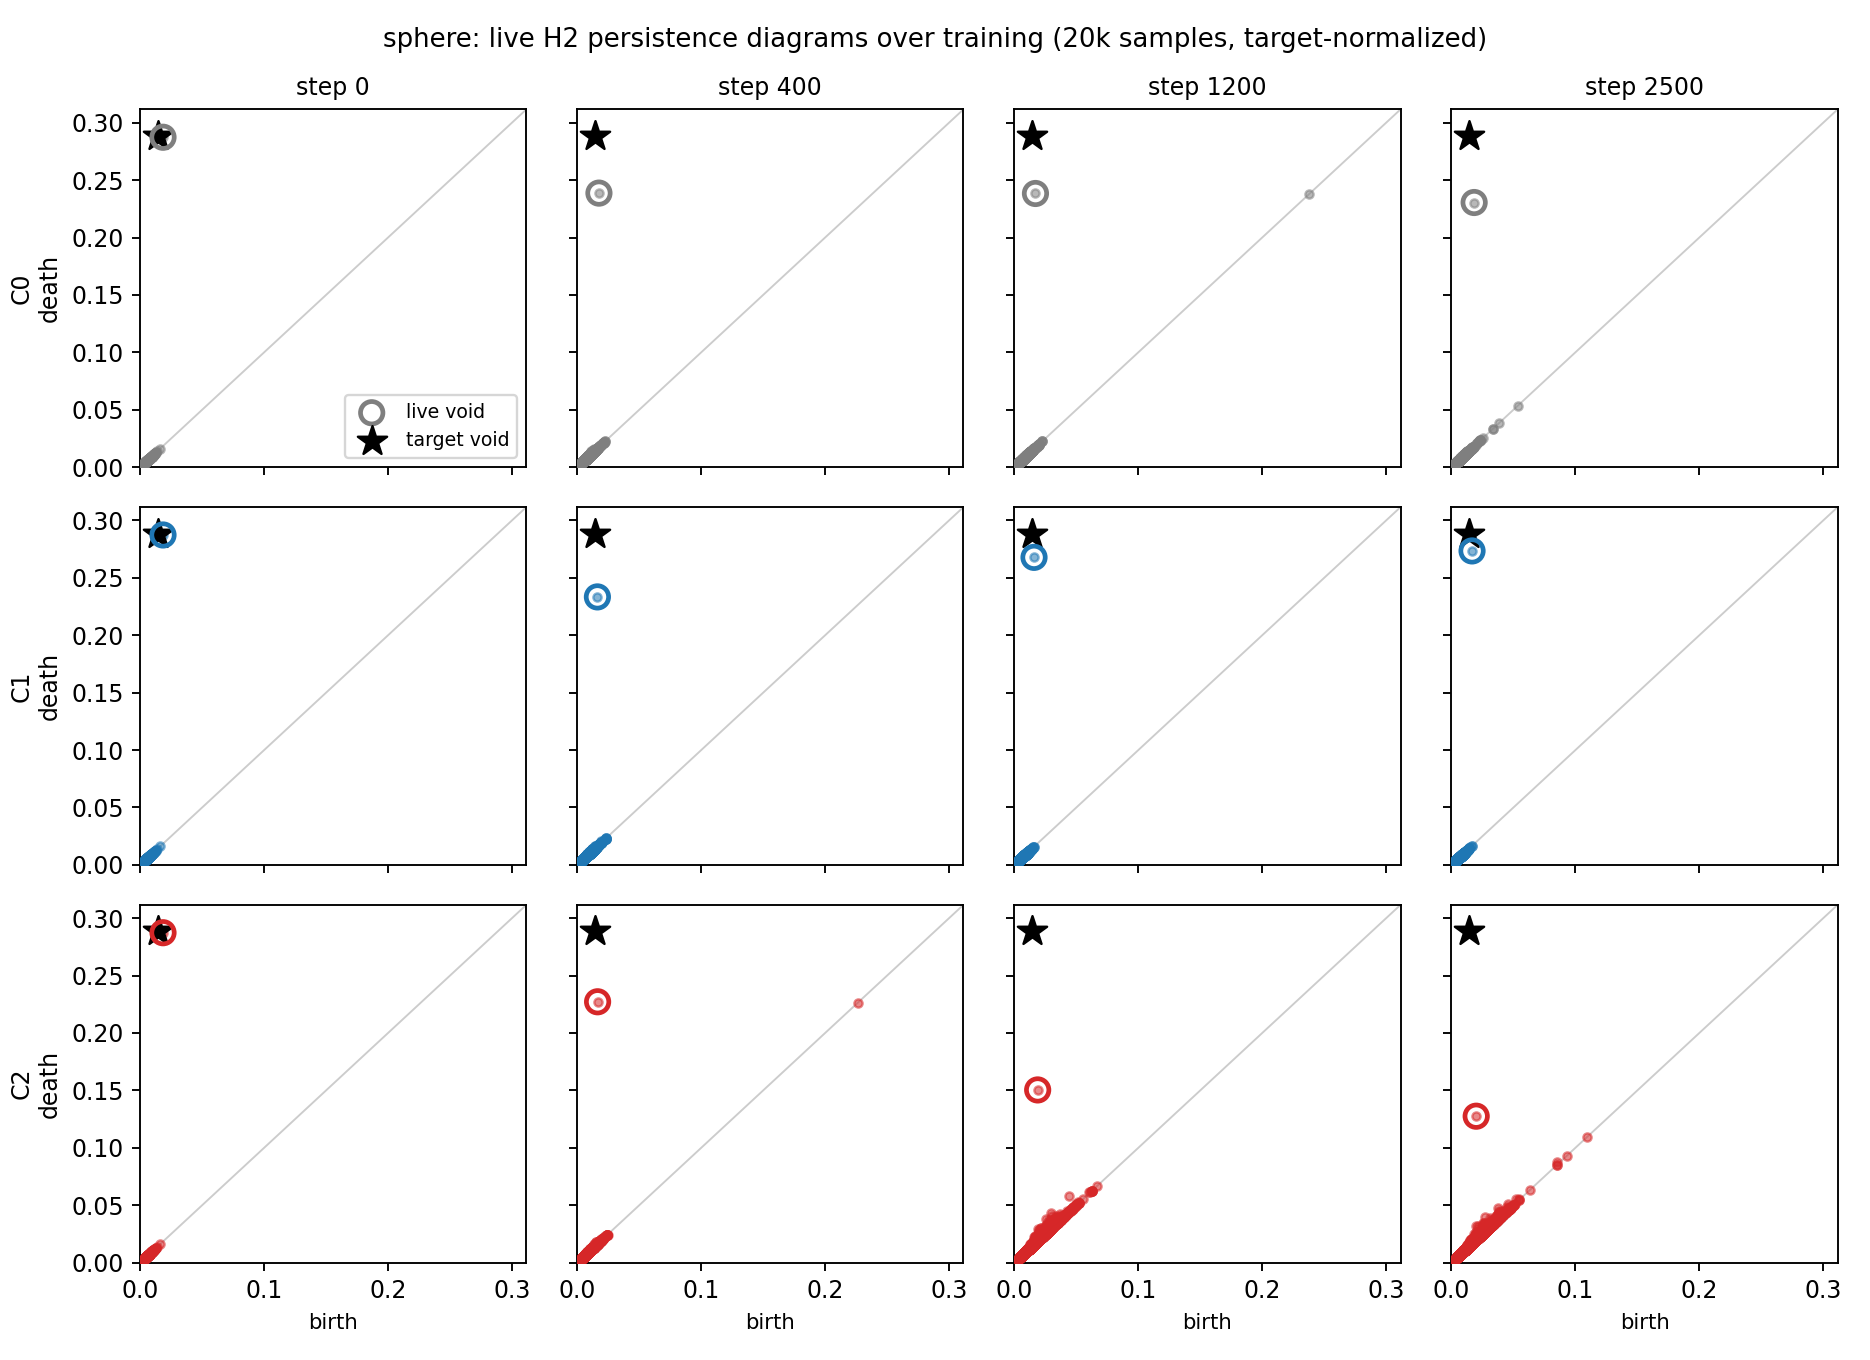
\includegraphics[width=\linewidth]{pd_trajectories.png}
\caption{Live H2 persistence diagrams over training (one sphere seed; 20k
samples, target-normalized; star $=$ target void bar, circle $=$ most
persistent live bar). \emph{Top}, baseline: the void drifts off target.
\emph{Middle}, loss: the void returns to the target once the ramp
activates. \emph{Bottom}, repulsion control: the void is pinned and
dragged away while near-diagonal phantom bars accumulate.}
\label{fig:pdtraj}
\end{figure}

\section{Additional result figures and the repair gate}
\label{app:extrafigs}

% Moved from the main paper's §5 for the 3DV page limit (2026-07-13):
% fig:gen (S2), fig:tails (S3), fig:nsig (S4), and the stage-3a gate
% figure fig:toys (S5) with its mechanism prose. Captions and % src
% comments carried over verbatim; the verdicts these figures illustrate
% are stated with their numbers in main-paper §5.
% Order note (2026-07-13 later): nsig moved BEFORE toys — same-class
% floats place in source order, and the tall toys figure was stranding
% nsig alone on a fourth page. S4/S5 swapped accordingly (main-text
% plain-text refs updated in results.tex).

Fig.~\ref{fig:gen} shows the generality-wave training trajectories
(main paper \S5.2, Table~2); Fig.~\ref{fig:tails} the per-seed tail
spread behind the sphere row of main-paper Table~1;
% (round-4 final numbering: main Table 1 = C-matrix, Table 2 = generality)
Fig.~\ref{fig:nsig} the torus significant-count check behind
\S5.1's zero-phantom-handles claim.

\begin{figure*}[t]
\centering
% src: topo3/report/{bob,fandisk}_series.png (topo_loss_report.py)
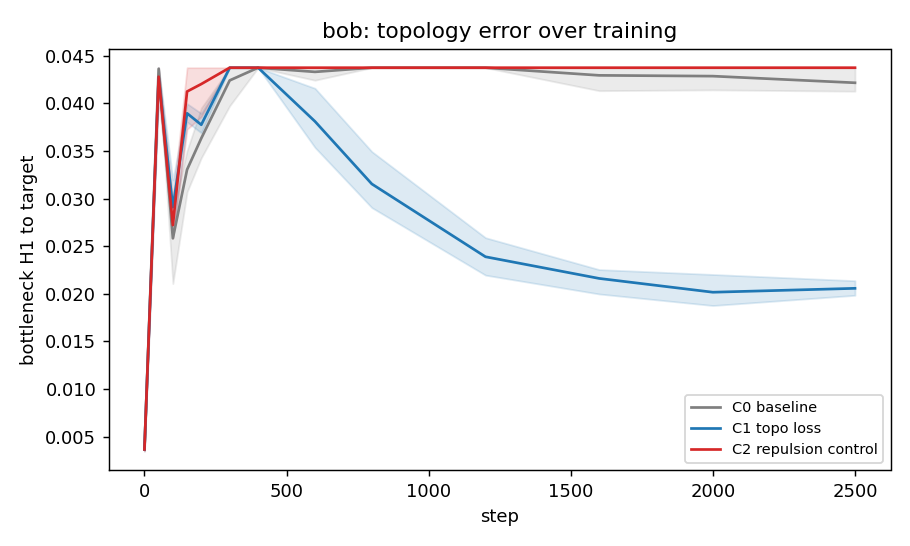
\includegraphics[width=0.495\linewidth]{bob_series.png}\hfill
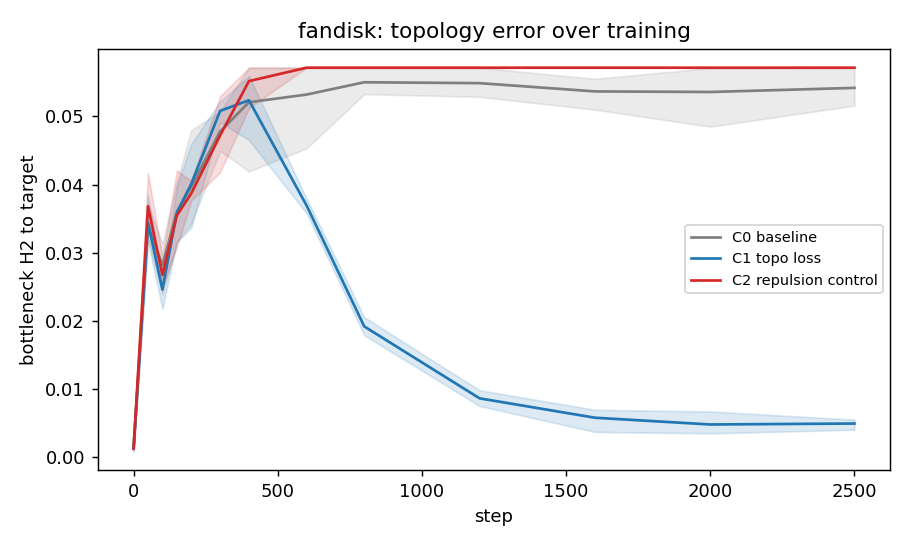
\includegraphics[width=0.495\linewidth]{fandisk_series.png}
\caption{Generality trajectories (line = seed mean, band = seed min--max).
\emph{Left}: bob (genus 1) --- the H1 result off the analytic family: the
loss halves the loop error with $\#$sig H1 $= 2$ in every seed, while the
control rides the baseline after collapsing a loop. \emph{Right}: fandisk
(CAD) --- the largest effect measured in this study ($10.4\times$).}
\label{fig:gen}
\end{figure*}

\begin{figure}[t]
\centering
% src: topo3/report/sphere_tail.png (per-seed tail means; results.json)
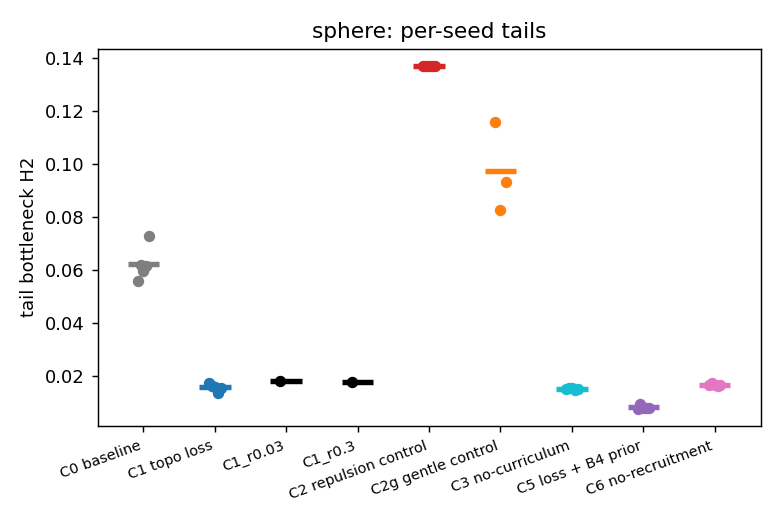
\includegraphics[width=0.9\linewidth]{sphere_tail.png}
\caption{Sphere, per-seed tail bottlenecks (dots) with arm means (bars).
Every loss arm sits far below baseline with tight seed spread; the two
control strengths bracket baseline from \emph{above}; the $\rho$ ablation
arms are indistinguishable from $\rho{=}0.1$.}
\label{fig:tails}
\end{figure}

\begin{figure}[t]
\centering
% src: topo3/report/torus_nsig.png (seed-mean significant-H1 count; axis
% clipped near target, off-scale init transient annotated on-plot)
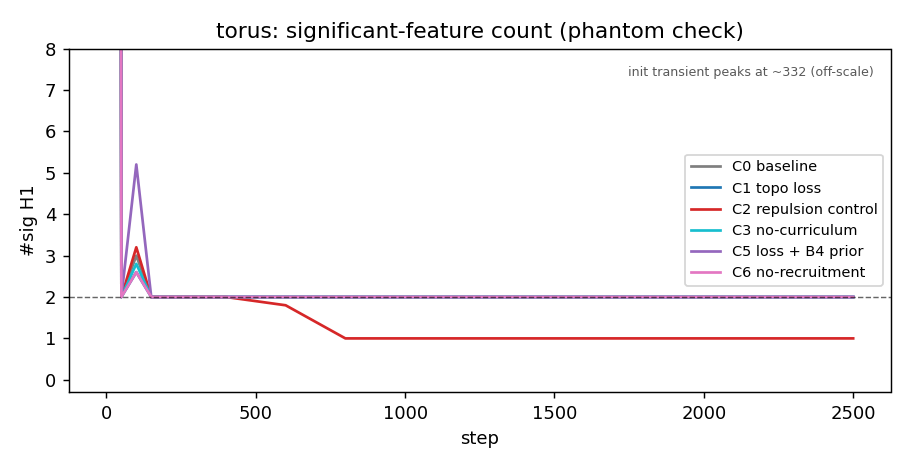
\includegraphics[width=0.85\linewidth]{torus_nsig.png}
\caption{Torus phantom check (main paper \S5.1): significant-H1 count over
training (seed means; dashed line: true $\beta_1{=}2$). After the brief
resampling transient near step 100, every loss arm sits exactly on two
significant loops --- zero phantom handles --- while the repulsion control
(C2) collapses a loop by step ${\sim}800$ and never recovers it.}
\label{fig:nsig}
\end{figure}

\paragraph{The stage-3a gate (main paper \S5).} Fig.~\ref{fig:toys} shows
three of the four repair probes run before integration: the loss alone
(no photometric term, Adam directly on point positions) must repair
defective clouds. The predicted location-blind pathology of recruitment
did not materialize, for a mechanism reason worth stating: tearing a
2-manifold shell cannot grow a component bar past the local detour scale
(the tug is abandoned), while cutting the 1-D bridge raises the recruited
bar's death monotonically toward target --- the runaway concentrates on
the only profitable direction.
% src: figures/phase3_toy/t{1..4}.json (PHASE3_PLAN.md Appendix A)

\begin{figure}[t]
\centering
% src: figures/phase3_toy/t{1,2,4}.png (tests/test_topo_loss.py artifacts;
% title bands cropped for print, panel data untouched; factors in t*.json)
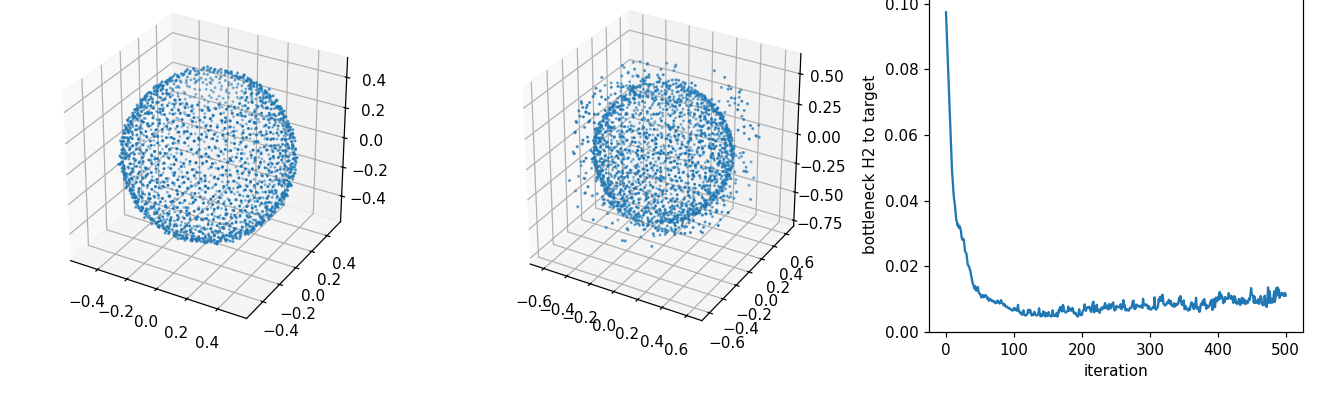
\includegraphics[width=\linewidth]{toy_t1.png}\\[2pt]
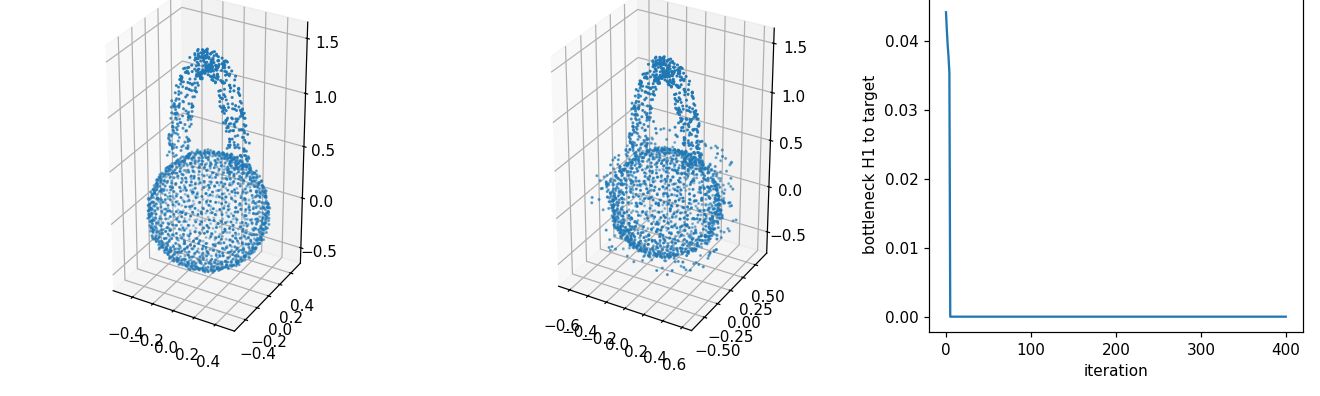
\includegraphics[width=\linewidth]{toy_t2.png}\\[2pt]
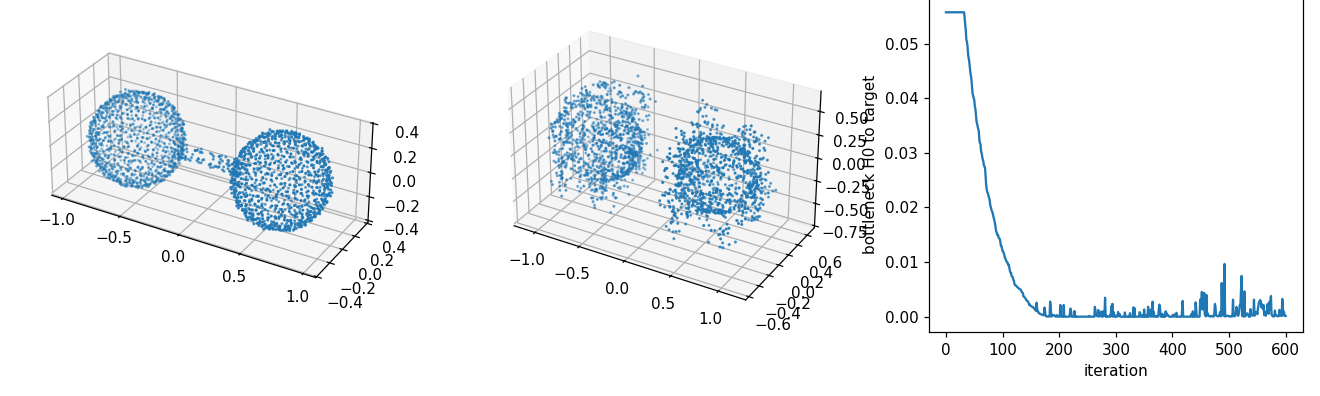
\includegraphics[width=\linewidth]{toy_t4.png}
\caption{The stage-3a gate: the loss alone (Adam on raw points, no
photometric term) repairs defective clouds; each row shows initial cloud,
final cloud, and bottleneck-to-target trajectory. \emph{Top} (T1):
punctured sphere --- the matched birth term closes the void ($8.8\times$).
\emph{Middle} (T2): spurious handle --- the diagonal term kills the extra
H1 bar. \emph{Bottom} (T4): bridged merge with no significant live H0 bar
--- recruitment severs the bridge ($450\times$, $\beta_0\,1{\to}2$), the
case where plain optimal matching provably has zero gradient. (T3,
mis-spaced components, $1229\times$: omitted for space.)}
\label{fig:toys}
\end{figure}

% Round-4 (2026-07-17): the decisive-shape trajectory figure moved here
% from main §5.1 (page budget for the round-4 teaser + qualitative
% matrix). Appended AFTER fig:toys so S2-S5 keep their numbers; this is
% Fig. S6. The full-width canvas also answers the review's Fig-1
% legibility note (many overlapping arms). Caption verbatim from main.
\begin{figure*}[t]
\centering
% src: topo3/report/{sphere,torus}_series.png (topo_loss_report.py; line =
% seed mean, band = seed min-max; underlying numbers in results.json)
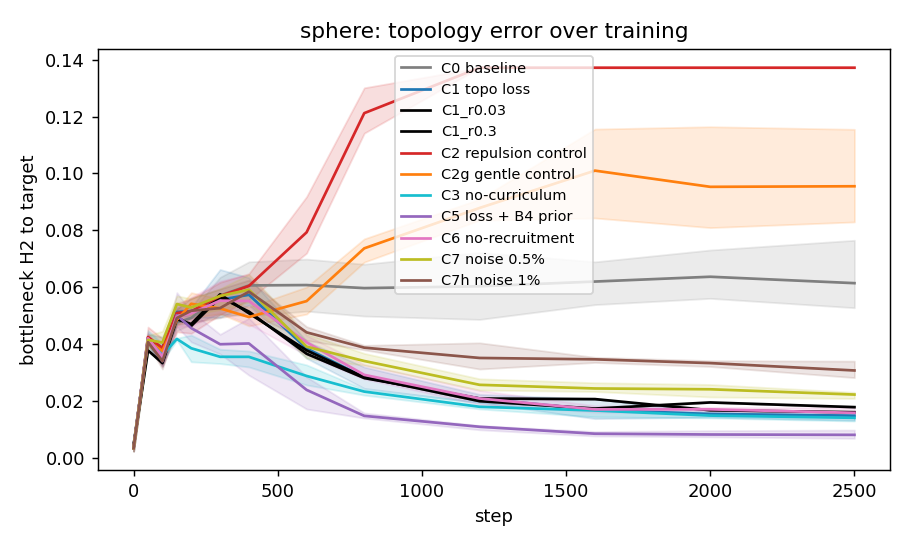
\includegraphics[width=0.495\linewidth]{sphere_series.png}\hfill
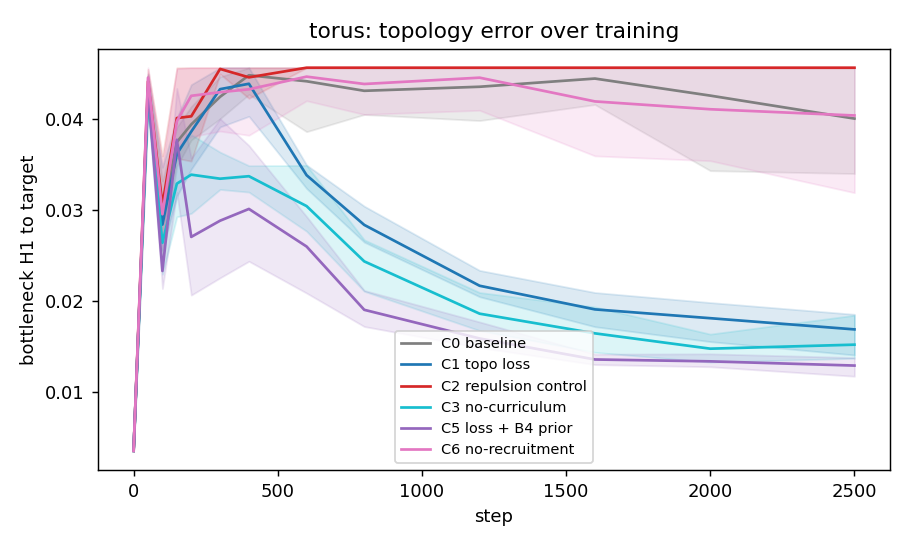
\includegraphics[width=0.495\linewidth]{torus_series.png}
\caption{Topology error over training: bottleneck to target in the
discriminating dimension (line = seed mean, band = seed min--max).
\emph{Left}, sphere (H2): every loss arm (C1, C3, C5, C6, both $\rho$
variants, noise pair C7/C7h) converges to a fraction of baseline; the
norm-matched repulsion control C2 is \emph{destructive}, and its gentle
variant C2g still ends worse than baseline. \emph{Right}, torus (H1), the
class no prior won: same ordering, C5 best; noise arms descend shallower
but never approach baseline; the no-recruitment ablation C6 rides it.}
\label{fig:mainseries}
\end{figure*}

% Round-4 (2026-07-17): fig:tomyum moved here from main §5.2 (page
% budget); appended after fig:mainseries so it is Fig. S7. The pot's
% showcase render re-enters main inside the qualitative matrix. Caption
% verbatim except the cross-doc \ref -> plain "main paper §4".
\begin{figure}[t]
\centering
% src: figures/tomyum_pot_alu{,_cut}.png (scripts/make_kinkin_figure.py ---
% CPU ray-traced render of the certified shell _meshes/kinkin_src.ply;
% aluminium material per advisor request 2026-07-11; rendered name
% tom-yum pot = internal asset name kinkin)
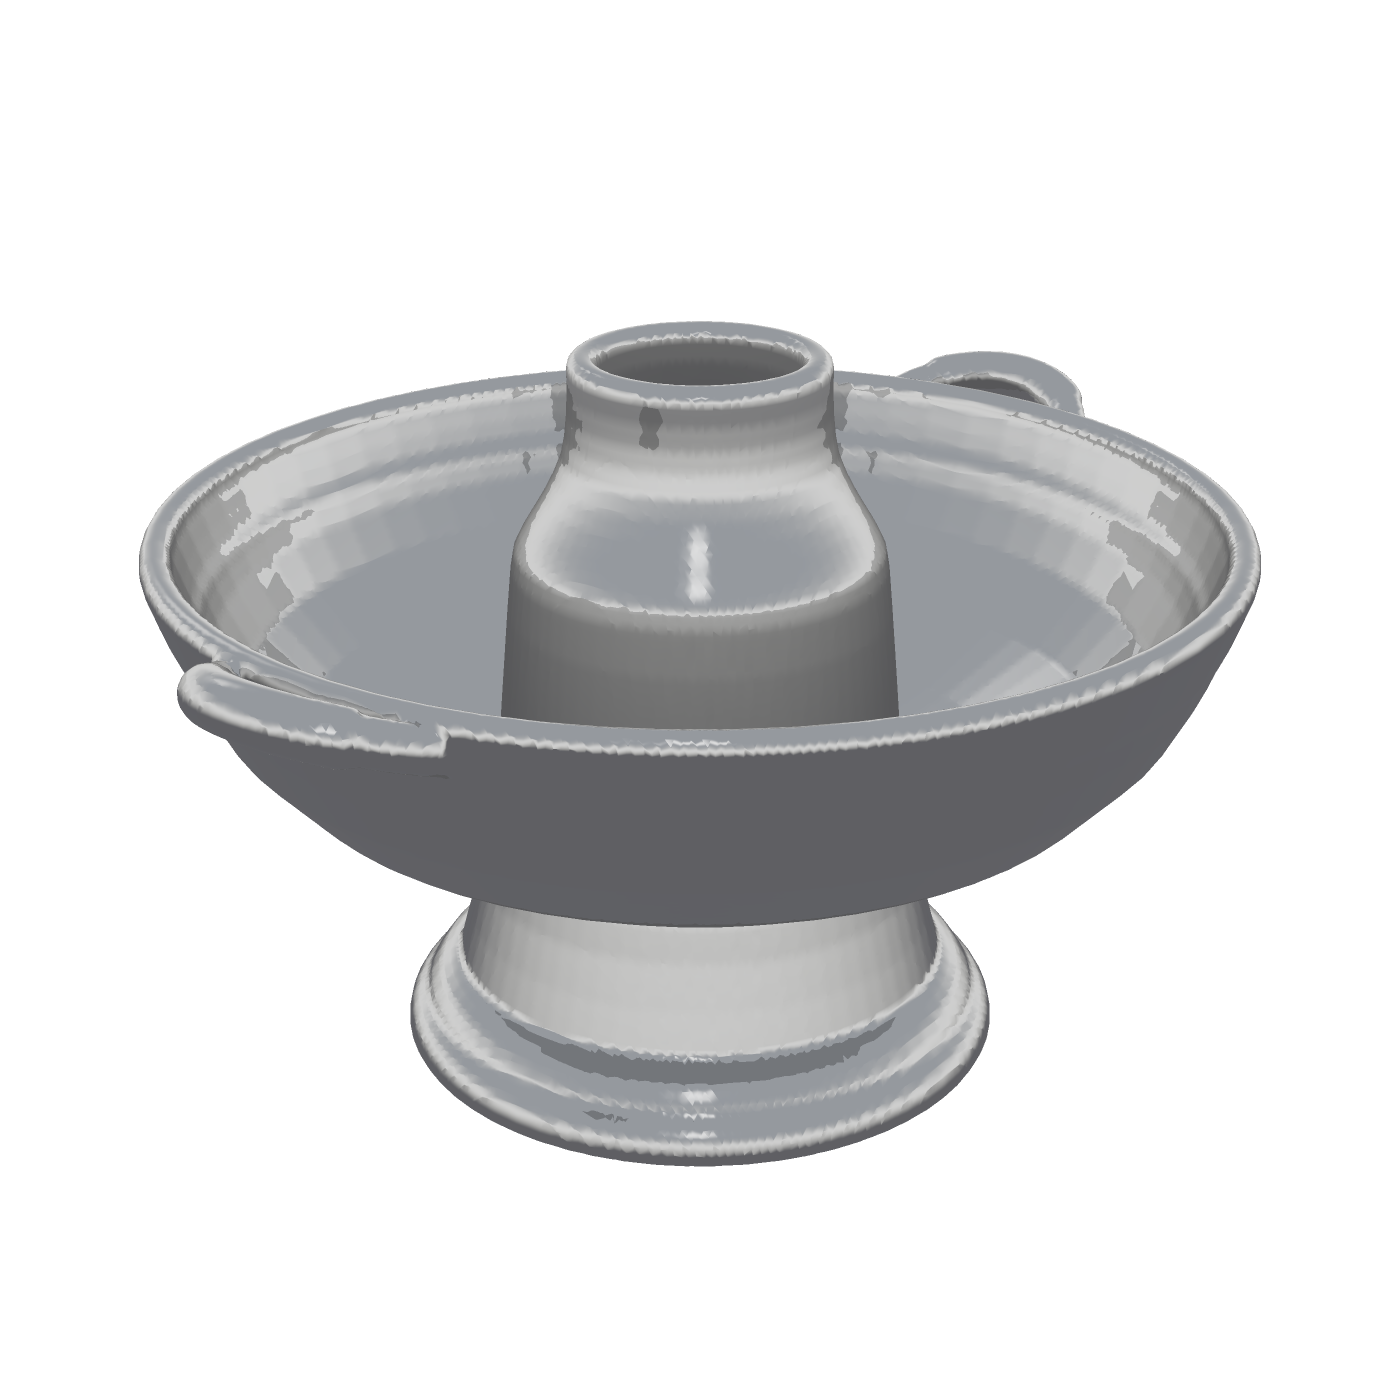
\includegraphics[width=0.365\linewidth]{tomyum_pot_alu.png}\hfill
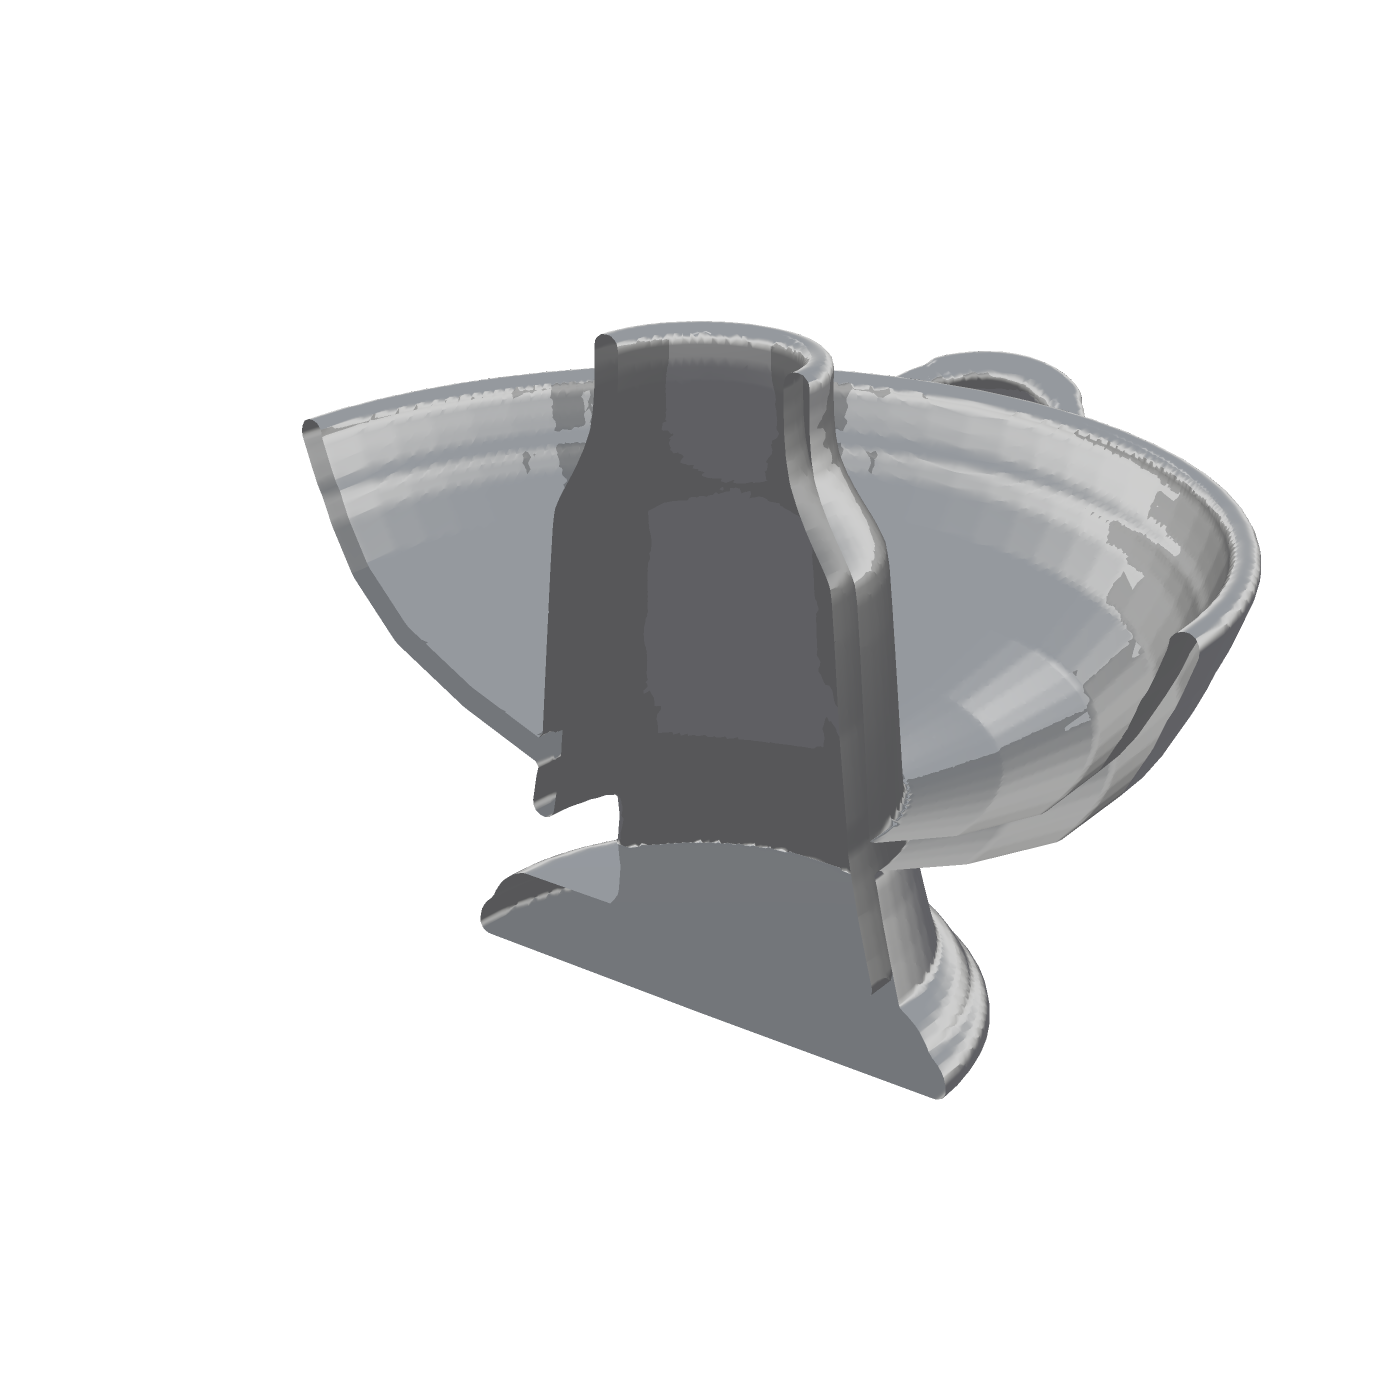
\includegraphics[width=0.365\linewidth]{tomyum_pot_alu_cut.png}
\caption{The \emph{tom-yum pot}: an artist-authored Blender model (raw
export: 9 open shells, 232 non-manifold junction edges) ingested and
certified to a single genus-3 shell, $\beta{=}(1,6,1)$ exact
(main paper \S4). \emph{Right}: cutaway --- the narrow flue mouth caps
at small $\alpha$, so the flue interior reads as an enclosed chamber: the
on-axis H2 void the floor rule selects at $M{=}8192$ (all H1 loops sit
below the floor).}
\label{fig:tomyum}
\end{figure}

% Round-4: the loop-class row of the qualitative matrix (main Fig. 1
% holds the two H2 rows under the page budget). Same renderer, badges,
% and camera discipline as Fig. 1; Fig. S8.
% src: scripts/make_matrix_figure.py (bob strip; seed-0 final_params.pt;
% badge = results.json nsig_final, identical across seeds)
\begin{figure*}[t]
\centering
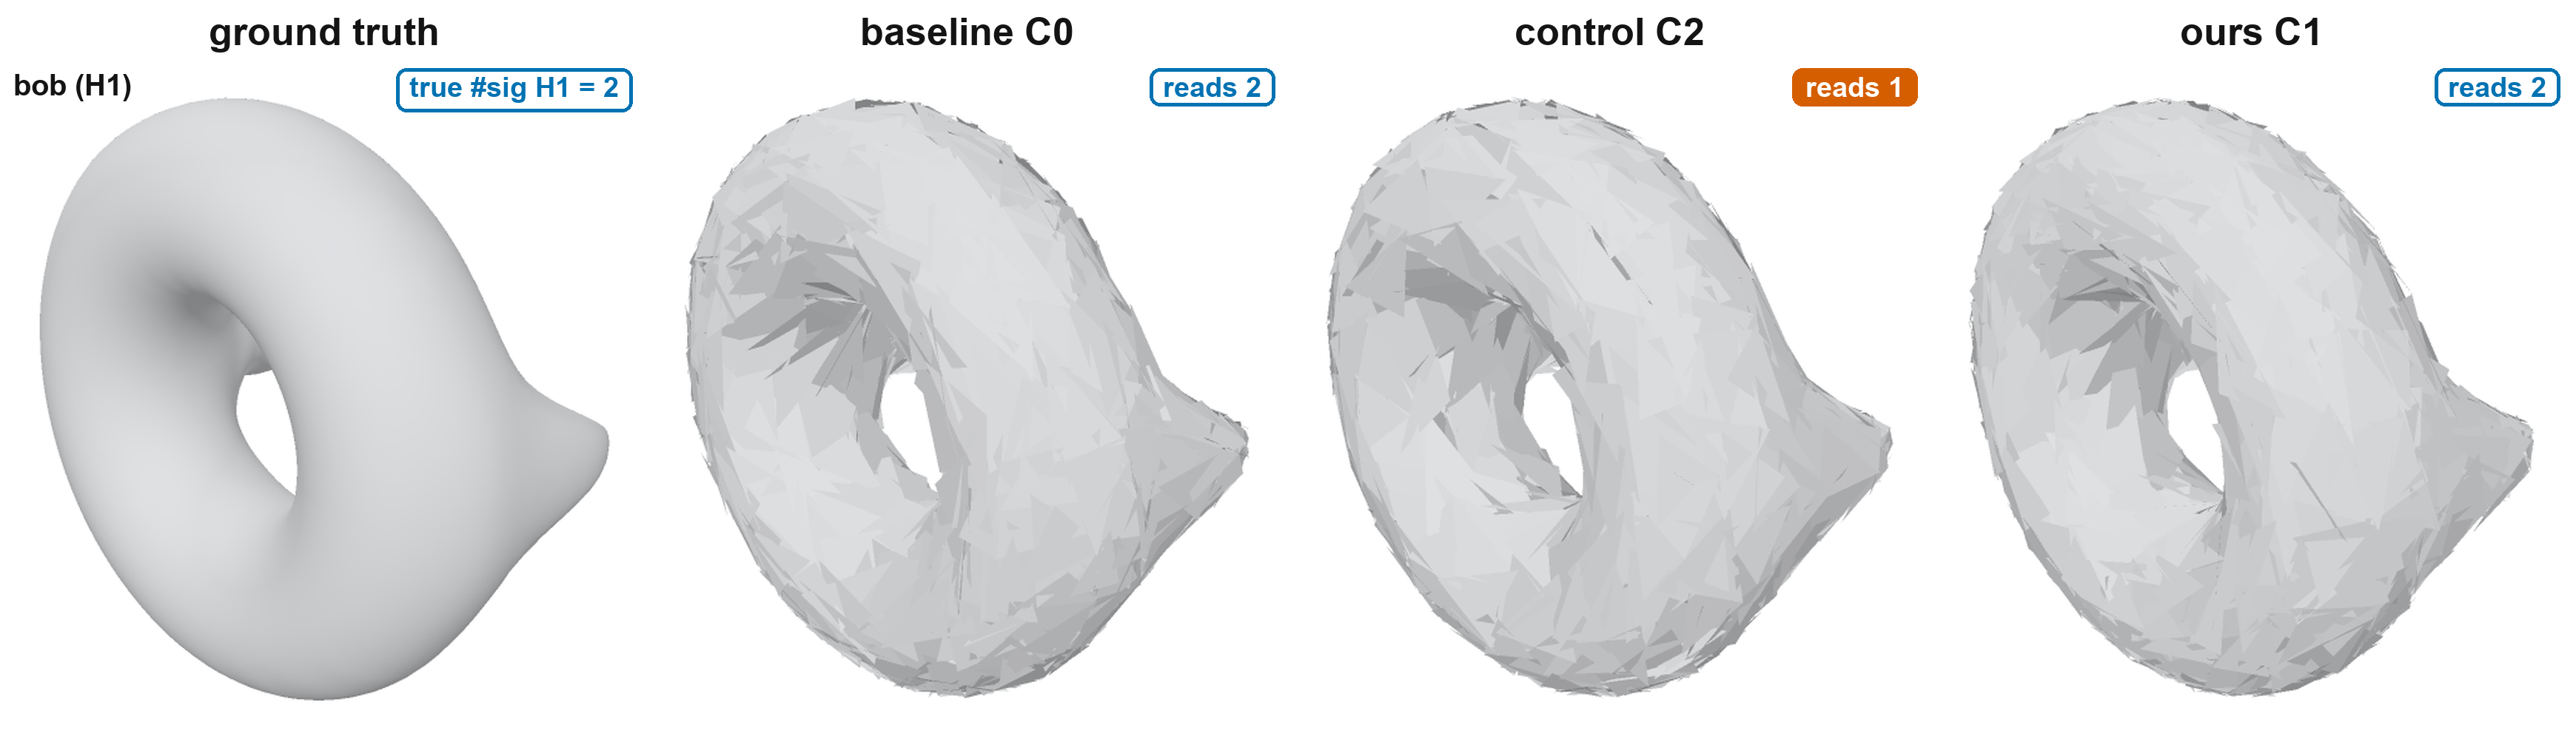
\includegraphics[width=0.9\linewidth]{matrix_bob.png}
\caption{The loop-class row of the main paper's Fig.~1 matrix: bob
(genus 1, H1). The repulsion control's reconstruction reads one
significant loop against the true two ($\beta_1\,2{\to}1$, all seeds)
at $2\times$ worse Chamfer, while baseline and loss both read two ---
the loss at half the baseline's tail error (main Table~2).}
\label{fig:bobmatrix}
\end{figure*}


\end{document}
